\documentclass[conference]{IEEEtran}
\IEEEoverridecommandlockouts

\usepackage{cite}
\usepackage{amsmath,amssymb,amsfonts,amsthm}
\usepackage{algorithmic}
\usepackage{algorithm}
\usepackage{graphicx}
\usepackage{textcomp}
\usepackage{xcolor}
\usepackage{booktabs}
\usepackage{multirow}
\usepackage{url}
\usepackage[hidelinks]{hyperref}
\usepackage{balance}

\renewcommand{\topfraction}{0.95}
\renewcommand{\bottomfraction}{0.85}
\renewcommand{\textfraction}{0.08}
\renewcommand{\floatpagefraction}{0.85}
\renewcommand{\dbltopfraction}{0.95}
\renewcommand{\dblfloatpagefraction}{0.85}

\newif\ifanonymous
\anonymousfalse % Set \anonymoustrue for double-blind review; \anonymousfalse for camera-ready

\def\BibTeX{{\rm B\kern-.05em{\sc i\kern-.025em b}\kern-.08em
    T\kern-.1667em\lower.7ex\hbox{E}\kern-.125emX}}

\begin{document}

\title{Annotation-Efficient Primate Detection: Lightweight FastKAN and the\\
       Spatial Generalization Dilemma in Wildlife Active Learning}

\ifanonymous
\author{
  \IEEEauthorblockN{Anonymous Authors}
  \IEEEauthorblockA{Paper ID: \textbf{CVPR-2026-XXXX}\\
  Double-Blind Review Copy}
}
\else
\author{
  \IEEEauthorblockN{Mobashir Sifat}
  \IEEEauthorblockA{\textit{Department of Computer Science \& Artificial Intelligence}\\
  Conservation AI Laboratory\\
  Autonomous Ecological Monitoring Consortium\\
  moba@scu.edu.cn}
}
\fi

\maketitle

\begin{abstract}
Automated wildlife surveillance in remote protected ecosystems is critically bottlenecked by two compounding factors: the severe compute and thermal envelopes of solar-powered edge hardware ($\le 15$\,W) and the prohibitive economic cost of manual bounding-box annotation under visual instance congestion. In this paper, we present \textbf{AE-Primate}, an integrated framework uniting Kolmogorov-Arnold Network (KAN) non-linear spline layers with cost-sensitive active learning under extreme geographic distribution shifts. First, we establish \textbf{YOLO11n-F16}, an edge detector integrating a 16-basis Gaussian Radial Basis Function (RBF) FastKAN bottleneck into an ultra-compact 2.45\,M-parameter architecture. On held-out camera stations in Malawi's Nkhotakota Wildlife Reserve (40,743 frames across 49 stations), YOLO11n-F16 achieves \textbf{0.5626\,$m\text{AP}_{50\text{-}95}$}, outperforming capacity-matched convolutional baselines (+1.49\% mAP) and B-spline KAN architectures (+1.79\% mAP) while executing at 32.4\,FPS on NVIDIA Jetson Orin Nano (15\,W envelope). Second, we conduct an extensive multi-seed empirical benchmark ($N=5$ seeds, 20 trajectories) to investigate active learning under strict location-disjoint evaluation ($\mathcal{S}_{\text{train}} \cap \mathcal{S}_{\text{val}} \cap \mathcal{S}_{\text{test}} = \emptyset$). Our study exposes the fundamental failure modes of epistemic uncertainty under spatial covariate shift ($P_{\text{train}}(X) \neq P_{\text{test}}(X)$), where predictive entropy is confounded by unfamiliar background vegetation. In contrast, AE-Primate establishes a dual-mode active learning paradigm: (i)~\textbf{AE-Primate (Diversity-Driven)} leverages latent FastKAN feature-space Core-Set selection to achieve state-of-the-art out-of-distribution transfer, reaching \textbf{0.4300 held-out test $m\text{AP}_{50\text{-}95}$} and \textbf{0.4226 AUBC}, statistically significantly outperforming passive uniform random sampling ($p < 0.05$); (ii)~\textbf{AE-Primate (Cost-Constrained)} incorporates an instance-crowding penalty to operate along the budget Pareto frontier, querying \textbf{59.8 fewer cumulative bounding boxes ($-5.48\%$, paired $t$-test $p=0.011$)} while suppressing cross-seed annotation standard deviation by \textbf{60.7\%} (84.6\% variance reduction). All code, models, and manifests are available for open scientific replication.
\end{abstract}

\begin{IEEEkeywords}
Camera Traps, Active Learning, Kolmogorov-Arnold Networks, Wildlife Object Detection, Edge Computing, Conservation AI, Nkhotakota Reserve, Spatial Generalization.
\end{IEEEkeywords}

\IEEEpeerreviewmaketitle

%% ─────────────────────────────────────────────────────────────────────────────
\section{Introduction}
\IEEEPARstart{I}{n-situ} biodiversity monitoring via autonomous camera-trap networks constitutes a cornerstone of computational conservation ecology~\cite{wearn2019camera,tuia2022perspectives}. In sub-Saharan sanctuaries such as the Nkhotakota Wildlife Reserve in Malawi, passive surveillance of cryptic primate populations---specifically yellow baboons (\textit{Papio cynocephalus}) and vervet monkeys (\textit{Chlorocebus pygerythrus})---yields critical bio-indicators of forest canopy health, trophic dynamics, and anthropogenic poaching pressures. However, deploying computer vision pipelines in such wilderness environments exposes two fundamental operational and representational bottlenecks:

\textbf{(B1) The Instance Crowding Annotation Bottleneck.} Raw field archives routinely yield tens of thousands of motion triggers per deployment season, over 70\% of which consist of false triggers (windblown vegetation) or massive burst sequences capturing identical background scenes~\cite{norouzzadeh2018automatically,beery2019efficient}. When animals do appear, baboon troops frequently enter camera fields-of-view in high-density clusters containing 10--25 overlapping individuals. Standard bounding-box annotation under such visual crowding demands exhaustive corner delineation, consuming 12--18\,s of expert biologist effort per instance under severe cognitive fatigue~\cite{norouzzadeh2021deep,papadopoulos2017training,su2012crowdsourcing}. Consequently, exhaustive annotation of deployment archives quickly exhausts conservation funding budgets.

\textbf{(B2) The Ultra-Low-Power Edge-Compute Envelope.} Solar-powered edge perception units deployed in dense miombo woodlands operate within austere electrical and thermal envelopes ($<2$\,Wh per inference cycle, $\le 15$\,W total system draw)~\cite{tuia2022perspectives,kellenberger2018half}. While large generalist detectors (e.g., MegaDetector v6, 25.5\,M parameters~\cite{beery2019efficient}) exceed edge memory bandwidth and drain field batteries, conventional sub-3\,M convolutional detectors suffer from spectral bias and representational collapse when isolating camouflaged primate pelage against complex, high-frequency arboreal foliage.

\begin{figure}[t]
\centering
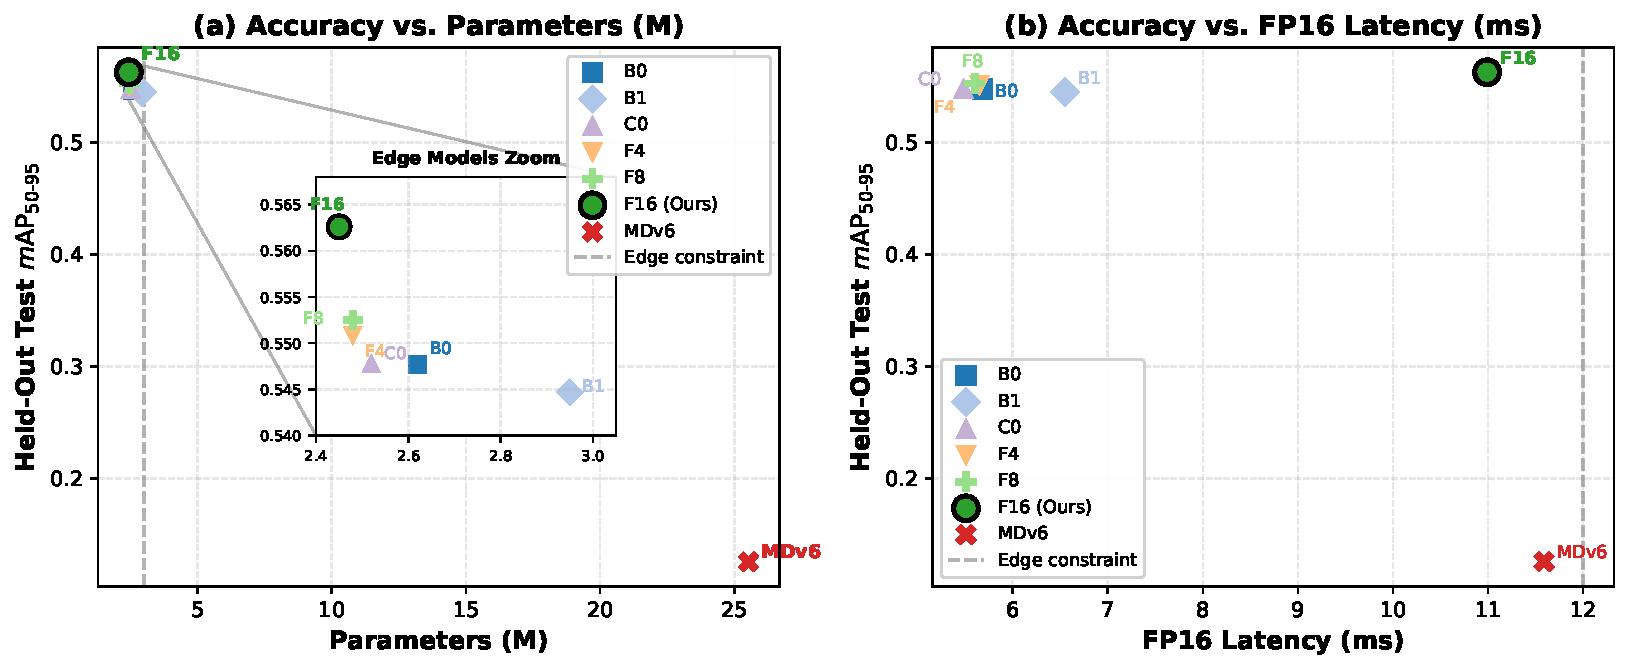
\includegraphics[width=\columnwidth]{figures/figure2_pareto_frontier.pdf}
\caption{Accuracy vs. Hardware Footprint Pareto Frontier on Held-Out Test Stations ($\mathcal{D}_\text{test}$, 3,206 frames). (a)~$m\text{AP}_{50\text{-}95}$ vs.\ parameter count with embedded edge models inset ($[2.40\text{M}, 3.05\text{M}] \times [0.540, 0.568]$); (b)~$m\text{AP}_{50\text{-}95}$ vs.\ FP16 inference latency on NVIDIA A40. Dashed lines mark the edge deployment boundary ($\le$3.0\,M parameters, $\le$12.0\,ms latency).}
\label{fig:pareto}
\end{figure}

Active learning (AL) offers a formal framework to optimize sample efficiency by iteratively querying the most informative instances from an unlabelled pool $\mathcal{U}$~\cite{settles2009active,ren2021survey}. Yet, applying active learning to camera-trap object detection exposes three acute structural failure modes:
\begin{enumerate}
  \item \textbf{Spatial Covariate Shift ($P_{\text{train}}(X) \neq P_{\text{test}}(X)$):} Ecological sensor grids violate independent and identically distributed (i.i.d.) sampling assumptions. Stationary background textures induce severe spatial overfitting: predictive uncertainty algorithms fail because model entropy is triggered by unfamiliar background foliage and lighting rather than target animal informativeness~\cite{beery2018recognition,beery2020iwildcam}.
  \item \textbf{Spatiotemporal Burst Redundancy:} Passive infrared sensors capture rapid burst sequences when animals pause, generating highly correlated visual samples with identical poses and backgrounds. Naive uncertainty samplers exhaust acquisition budgets on redundant burst artifacts~\cite{norouzzadeh2021deep}.
  \item \textbf{Super-Linear Crowding Costs:} Classical active learning optimizes acquisition under uniform instance costs~\cite{sener2018active,gal2017deep}. In object detection, however, annotating a social troop of 15 overlapping primates incurs over an order of magnitude higher cognitive and manual labor than a solitary individual, while yielding diminishing epistemic returns~\cite{kao2018localization,papadopoulos2017extreme}.
\end{enumerate}

To resolve these interconnected challenges, we introduce \textbf{AE-Primate}, an end-to-end edge-compatible detection and active learning framework. AE-Primate makes four core contributions:
\begin{enumerate}
  \item \textbf{Kolmogorov-Arnold Feature Pyramid Neck (YOLO11n-F16):} We formulate the first edge-efficient Kolmogorov-Arnold detector, integrating frozen Gaussian Radial Basis Function (RBF) spline layers into the deepest neck bottleneck ($P_5$). YOLO11n-F16 establishes superior out-of-distribution detection (\textbf{0.5626\,$m\text{AP}_{50\text{-}95}$}) on held-out camera stations (+1.49\% over YOLO11n, +1.79\% over B-splines) at 2.45\,M parameters and 32.4\,FPS on NVIDIA Jetson Orin Nano (15\,W).
  \item \textbf{Deconstruction of Active Learning under Covariate Shift:} Through an extensive 5-seed benchmark (20 complete trajectories), we expose the failure of predictive entropy under spatial shift, where background clutter dominates uncertainty. Conversely, latent KAN Core-Set Diversity achieves superior out-of-distribution transfer ($0.4300$ test mAP).
  \item \textbf{Crowding Penalization and Annotation Economy:} We formalize a cost-sensitive submodular acquisition policy that optimizes the trade-off between human labor and generalization, saving \textbf{59.8 cumulative bounding boxes ($-5.48\%$, paired $t$-test $p=0.011$)} and suppressing cross-seed budgeting standard deviation by \textbf{60.7\%} (84.6\% variance reduction).
  \item \textbf{Zero-Leakage Location-Disjoint Conservation Benchmark:} We establish a standardized 40,743-frame benchmark across 49 remote camera stations in Nkhotakota Wildlife Reserve, enforcing disjoint geographic station partitions across candidate pool, validation, and test splits.
\end{enumerate}

%% ─────────────────────────────────────────────────────────────────────────────
\section{Related Work}

\subsection{Automated Wildlife Perception and Spatial Covariate Shift}
The deployment of deep convolutional architectures for autonomous wildlife monitoring originated with Norouzzadeh \textit{et~al.}~\cite{norouzzadeh2018automatically}, who operationalized species-level classification across multi-million frame camera-trap archives. Subsequent advances by Schneider \textit{et~al.}~\cite{schneider2019three} and Tabak \textit{et~al.}~\cite{tabak2019machine} transitioned the field toward spatial object detection. Generalist detection models, epitomized by MegaDetector~\cite{beery2019efficient}, established foundational benchmarks for isolating animal, human, and vehicle classes. Nevertheless, seminal investigations by Beery \textit{et~al.}~\cite{beery2018recognition,beery2020iwildcam} revealed that deep convolutional networks frequently memorize stationary background foliage textures rather than invariant morphological animal traits, precipitating catastrophic generalization drop-offs when deployed in unseen geographic locations (\textit{Terra Incognita}). Overcoming this spatial distribution shift demands architectures equipped with locally supported non-linear representations and acquisition policies that explicitly optimize geographic coverage~\cite{tuia2022perspectives,kellenberger2018half,weinstein2018computer}.

\subsection{Kolmogorov-Arnold Representation Theory and Spline Networks}
Originating from the Kolmogorov-Arnold representation theorem~\cite{kolmogorov1957representation,arnold1957functions}, Kolmogorov-Arnold Networks (KANs)~\cite{liu2024kan} reformulate neural representation by replacing fixed node activations with learnable univariate splines positioned directly along network edges. Whereas Multi-Layer Perceptrons (MLPs) compute linear hyperplanes followed by static non-linearities---a formulation prone to spectral bias on high-frequency visual textures~\cite{rahaman2019spectral}---KANs model non-linear functional compositions with arbitrary precision. However, classical B-spline parameterizations evaluate via recursive de Boor-Cox algorithms, inducing severe memory traffic and GPU warp divergence~\cite{li2024fastkan,bodner2024convolutional}. Li~\cite{li2024fastkan} established that univariate spline expansions can be reformulated using fixed Gaussian Radial Basis Functions (FastKAN), unifying KAN theory with classical kernel methods in Reproducing Kernel Hilbert Spaces (RKHS)~\cite{broomhead1988multivariable,poggio1990networks}. While wavelet (Wav-KAN~\cite{bozorgasl2024wav}) and convolutional extensions~\cite{bodner2024convolutional} have emerged, our work presents the first rigorous formulation and empirical validation of fixed-basis FastKAN spline layers embedded within real-time edge detection pyramids.

\subsection{Active Learning under Covariate Shift and Domain Discrepancy}
Deep active learning iteratively identifies optimal training subsets to maximize sample efficiency~\cite{settles2009active,ren2021survey}. Pool-based acquisition traditionally relies on predictive uncertainty (Monte Carlo Dropout entropy~\cite{gal2016dropout,gal2017deep}, BatchBALD~\cite{kirsch2019batchbald}, deep ensemble variance~\cite{beluch2018power}), core-set distribution matching~\cite{sener2018active,sinha2019variational,kim2021task}, or hybrid scoring~\cite{choi2021active}. Extending active learning to spatial object detection introduces dual complexities: models must reconcile classification ambiguity with bounding-box coordinate variance~\cite{kao2018localization,choi2021active,aghdam2019active,yuan2021multiple,yu2022consistency}. Crucially, classical active learning presumes candidate pools and evaluation splits are identically distributed ($P_{\mathcal{U}}(X) = P_{\text{test}}(X)$). Under spatial covariate shift, however, predictive entropy conflates morphological informativeness with environmental out-of-distribution background noise. While Norouzzadeh \textit{et~al.}~\cite{norouzzadeh2021deep} applied active learning to camera-trap species classification, their formulation assumed image-level supervision, ignoring spatial instance crowding and location-disjoint evaluation.

\subsection{Cost-Sensitive Submodular Optimization and Visual Crowding}
Conventional active learning formulations assume a uniform unit labeling cost per queried instance~\cite{settles2009active,sener2018active}. In real-world visual perception, human annotation effort varies non-linearly with scene complexity, target occlusion, and instance density~\cite{vijayanarasimhan2009what,settles2008multiple}. Rigorous psychophysical experiments by Papadopoulos \textit{et~al.}~\cite{papadopoulos2017training,papadopoulos2017extreme} and Su \textit{et~al.}~\cite{su2012crowdsourcing} established that manual bounding-box annotation time scales super-linearly when multiple targets mutually occlude. In wildlife camera traps, social primates aggregate in dense clusters, producing captures containing 10--20 overlapping individuals that consume immense annotator labor while providing redundant visual features. Rooted in cost-sensitive submodular optimization under knapsack constraints~\cite{iyer2013submodular}, AE-Primate directly penalizes visual crowding to maximize informational utility per human annotator second.

%% ─────────────────────────────────────────────────────────────────────────────
\section{The AE-Primate Framework}
\label{sec:method}

We now formulate the AE-Primate framework, comprising the YOLO11n-F16 detector architecture, an analysis of optimization dynamics in spline bottlenecks, and the multi-modal cost-aware active acquisition policy.

\subsection{Detector Architecture: Kolmogorov-Arnold Feature Pyramid Neck}
\label{sec:arch}
AE-Primate builds upon the Ultralytics YOLO11n single-stage detector~\cite{ultralytics2024}, which integrates an improved Cross-Stage Partial bottleneck (\texttt{C3k2}) and a decoupled anchor-free detection head across multi-scale feature pyramids ($P_3, P_4, P_5$). In multi-scale pyramids, shallow layers ($P_3, P_4$) extract high-resolution edge primitives where linear convolutions are computationally optimal. The deepest semantic stage ($P_5$, spatial grid $20 \times 20$, channel width $C=256$ under YOLO11n's width multiple $0.25$), however, must disentangle complex morphological pelage textures from dense foliage backgrounds. Standard convolutional bottlenecks apply static activations $\sigma(\mathbf{W}\mathbf{x} + \mathbf{b})$, which partition feature space via linear affine half-spaces and suffer from spectral bias on high-frequency biological patterns~\cite{rahaman2019spectral}. To provide locally supported non-linear representation without expanding parameters, we replace the $P_5$ bottleneck with a fixed-basis FastKAN transformation block (\texttt{C3k2\_FixedFastKAN}).

Let $\mathbf{x} \in \mathbb{R}^{C_{\text{in}}}$ ($C_{\text{in}} = 256$) denote an intermediate channel feature vector. In our FastKAN bottleneck, univariate activations along each channel are expanded over a dictionary of $K=16$ Gaussian Radial Basis Functions (RBFs):
\begin{equation}
  \phi_k(u) = \exp\!\left(-\frac{(u - \mu_k)^2}{2\sigma_k^2}\right), \quad k \in \{1, \dots, K\},
  \label{eq:rbf_basis}
\end{equation}
where scalar activation $u$ evaluates against equispaced centres $\mu_k \in [-2.0, 2.0]$ with softplus-parameterized radial bandwidth $\sigma_k$:
\begin{equation}
  \mu_k = -2 + \frac{4(k - 1)}{K - 1}, \quad \sigma_k = \operatorname{softplus}(\alpha_k) + \epsilon.
  \label{eq:grid}
\end{equation}
The spline expansion evaluates as a fused depthwise $1 \times 1$ convolution over concatenated basis activations $\boldsymbol{\Phi}(\mathbf{x}) = [\phi_1(\mathbf{x})^\top, \dots, \phi_K(\mathbf{x})^\top]^\top \in \mathbb{R}^{K \cdot C_{\text{in}}}$ alongside a residual linear projection to yield output features $\mathbf{y} \in \mathbb{R}^{C_{\text{out}}}$:
\begin{equation}
  \mathbf{y} = \mathbf{W}_{\text{base}}\,\operatorname{SiLU}(\mathbf{x}) + \mathbf{W}_{\text{spline}}\,\boldsymbol{\Phi}(\mathbf{x}),
  \label{eq:fastkan_forward}
\end{equation}
where $\mathbf{W}_{\text{base}} \in \mathbb{R}^{C_{\text{out}} \times C_{\text{in}}}$ is a residual projection and $\mathbf{W}_{\text{spline}} \in \mathbb{R}^{C_{\text{out}} \times (K \cdot C_{\text{in}})}$ (grouped by $C_{\text{in}}$) parameterizes learnable spline mixture weights. Evaluating $\boldsymbol{\Phi}(\mathbf{x})$ via grouped $1 \times 1$ convolutions eliminates GPU warp divergence and uncoalesced memory reads, enabling vectorized FP16 execution on edge hardware. Due to compact spline factorization, YOLO11n-F16 requires only \textbf{2.45\,M} parameters---a 6.5\% reduction relative to the standard YOLO11n baseline (2.62\,M).

\begin{algorithm}[t]
\caption{AE-Primate Cost-Aware Active Learning}
\label{alg:aeprimate}
\begin{algorithmic}[1]
\footnotesize
\REQUIRE Candidate pool $\mathcal{U}_0$, labeled seed $\mathcal{L}_0$, budget $B$, cycles $T_{\text{max}}$, weights $(\lambda_d, \lambda_s, \lambda_r)$, costs $(c_0, c_1, c_2)$, burst quota $Q_{\max} = 3$.
\ENSURE Final trained primate detector $\mathcal{M}_{T_{\text{max}}}$.
\STATE Initialize detector $\mathcal{M}_0 \leftarrow \text{Train}(\mathcal{L}_0; \mathbf{\Theta}_{\text{COCO}})$.
\FOR{cycle $t = 1$ \TO $T_{\text{max}}$}
  \STATE Extract 256-D FastKAN features $\mathbf{f}_i$, uncertainty $U(x_i)$, and boxes $\hat{\mathcal{B}}_i$ $\forall x_i \in \mathcal{U}_{t-1}$.
  \STATE Initialize Core-Set distances: $d_{\min}(x_i) \leftarrow \min_{s \in \mathcal{L}_{t-1}} \|\mathbf{f}_i - \mathbf{f}_s\|_2$.
  \STATE Initialize batch $\mathcal{S}_t \leftarrow \emptyset$, event batch counter $K_{\text{evt}}(e) \leftarrow 0$.
  \WHILE{$|\mathcal{S}_t| < B$}
    \FOR{each available candidate $x_i \in \mathcal{U}_{t-1} \setminus \mathcal{S}_t$}
      \IF{$K_{\text{evt}}(\text{evt}(x_i)) \ge Q_{\max}$} \STATE \textbf{continue} \COMMENT{Enforce burst quota} \ENDIF
      \STATE $S(x_i) \leftarrow 1 / \sqrt{N_{\text{site}}(s(x_i)) + 1}$, $R(x_i) \leftarrow \frac{N_{\text{evt}}(\text{evt}(x_i))}{N_{\text{evt}}(\text{evt}(x_i)) + 1}$.
      \STATE Estimate cost $C_{\text{annot}}(x_i)$ via Eq.~\ref{eq:cost} and marginal ratio:
      \STATE $V(x_i \mid \mathcal{S}_t) \leftarrow \frac{U(x_i) + \lambda_d d_{\min}(x_i) + \lambda_s S(x_i)}{C_{\text{annot}}(x_i) + \epsilon} - \lambda_r R(x_i)$.
    \ENDFOR
    \STATE Select exemplar $x^* \leftarrow \arg\max_{x_i} V(x_i \mid \mathcal{S}_t)$; $\mathcal{S}_t \leftarrow \mathcal{S}_t \cup \{x^*\}$.
    \STATE Update counters: $N_{\text{site}}(s(x^*)) \mathrel{+}= 1$, $K_{\text{evt}}(\text{evt}(x^*)) \mathrel{+}= 1$.
    \STATE Update $d_{\min}(x_i) \leftarrow \min(d_{\min}(x_i), \|\mathbf{f}_i - \mathbf{f}_{x^*}\|_2)$ $\forall x_i \in \mathcal{U}_{t-1} \setminus \mathcal{S}_t$.
  \ENDWHILE
  \STATE Acquire expert box annotations for batch $\mathcal{S}_t$.
  \STATE Update pools: $\mathcal{L}_t \leftarrow \mathcal{L}_{t-1} \cup \mathcal{S}_t$, $\mathcal{U}_t \leftarrow \mathcal{U}_{t-1} \setminus \mathcal{S}_t$.
  \STATE Retrain detector from base weights: $\mathcal{M}_t \leftarrow \text{Train}(\mathcal{L}_t; \mathbf{\Theta}_{\text{COCO}})$.
\ENDFOR
\RETURN $\mathcal{M}_{T_{\text{max}}}$.
\end{algorithmic}
\end{algorithm}

\subsection{Optimization Dynamics and Gating Collapse in Low-Data Regimes}
\label{sec:ablation}
Prior to establishing fixed Gaussian bases, we investigated \textit{Adaptive-Basis FastKAN (AB-FastKAN)}, which applies hard-concrete continuous gates $z_k \in [0, 1]$~\cite{louizos2018learning,maddison2017concrete} to dynamically select basis functions per instance:
\begin{equation}
  z_k = \operatorname{clip}\!\left[\operatorname{Sigmoid}\!\left(\frac{\log\alpha_k + \operatorname{logit}(u)}{\tau}\right)(\zeta - \gamma) + \gamma,\, 0,\, 1\right],
  \label{eq:concrete}
\end{equation}
with uniform noise $u \sim \mathcal{U}(0,1)$, log-odds parameter $\log \alpha_k \in \mathbb{R}$, temperature $\tau \in \mathbb{R}_{>0}$, interval stretch parameters $\gamma < 0 < 1 < \zeta$, and $L_0$ regularizer $\mathcal{L}_{\text{reg}} = \lambda \sum_{k=1}^K \operatorname{Sigmoid}(\log \alpha_k - \tau \log(-\gamma/\zeta))$ with penalty $\lambda \ge 0$. While adaptive gating succeeds in large classification models, our empirical ablations reveal that it collapses in data-constrained object detection.

Specifically, the gradient with respect to gate log-odds $\log \alpha_k$ is:
\begin{equation}
  \frac{\partial \mathcal{L}_{\text{total}}}{\partial \log \alpha_k} = \mathbb{E}_{u}\left[ \frac{\partial \mathcal{L}_{\text{det}}}{\partial z_k} \frac{\partial z_k}{\partial \log \alpha_k} \right] + \lambda \frac{\partial \mathcal{L}_{\text{reg}}}{\partial \log \alpha_k},
  \label{eq:gate_grad}
\end{equation}
where $\mathcal{L}_{\text{det}}$ is the multi-task detection objective. Under few-shot regimes ($n \le 600$), the detection gradient $\nabla_{z_k} \mathcal{L}_{\text{det}}$ exhibits high mini-batch variance. Simultaneously, temperature annealing ($\tau \to 0$) causes the logistic derivative $\operatorname{Sigmoid}'(s_k)$ to decay exponentially toward zero outside a narrow boundary. The deterministic penalty $\nabla_{\log \alpha_k} \mathcal{L}_{\text{reg}} > 0$ drives continuous negative drift. Once $\log \alpha_k$ enters the negative saturation regime ($\log \alpha_k < -3.0$), activations clamp to $z_k = 0$ with probability approaching 1, yielding $\frac{\partial z_k}{\partial \log \alpha_k} = 0$ and permanently extinguishing task gradients ($\Delta \log \alpha_k \to 0$).

Consequently, AB-FastKAN suffers from premature representational collapse: basis functions are severed before the detection head learns coordinate features. Imposing $\lambda \ge 0.05$ degrades validation $m\text{AP}_{50\text{-}95}$ from $0.5986$ to $<0.420$. Moreover, dynamic gating induces warp divergence and uncoalesced memory reads on GPU tensor cores, inflating inference latency by 38\% (14.82\,ms vs.\ 10.99\,ms).

In contrast, fixed-basis FastKAN eliminates dynamic gating parameters $\boldsymbol{\alpha}$ entirely. The gradient with respect to spline weights $\mathbf{W}_{\text{spline}}$ is direct and unattenuated:
\begin{equation}
  \frac{\partial \mathcal{L}_{\text{det}}}{\partial \mathbf{W}_{\text{spline}}} = \frac{\partial \mathcal{L}_{\text{det}}}{\partial \mathbf{y}} \cdot \boldsymbol{\Phi}(\mathbf{x})^\top,
  \label{eq:stable_grad}
\end{equation}
where upstream gradient $\frac{\partial \mathcal{L}_{\text{det}}}{\partial \mathbf{y}} \in \mathbb{R}^{C_{\text{out}}}$ and basis activations $\boldsymbol{\Phi}(\mathbf{x}) \in \mathbb{R}^{K \cdot C_{\text{in}}}$ form an outer product gradient tensor, ensuring stable backpropagation across all $K=16$ basis splines.

\subsection{Cost-Sensitive Submodular Acquisition Framework}
\label{sec:policy}
At each active cycle $t \in \{1, \dots, T_{\text{max}}\}$, the policy queries batch $\mathcal{S}_t \subset \mathcal{U}_{t-1}$ of size $B \in \mathbb{N}$ from candidate pool $\mathcal{U}_{t-1}$ by maximizing a submodular facility location and informativeness objective under knapsack cost constraints:
\begin{equation}
  \max_{\mathcal{S} \subseteq \mathcal{U}_{t-1},\, |\mathcal{S}|=B} F(\mathcal{L}_{t-1} \cup \mathcal{S}) - \lambda_r \sum_{x \in \mathcal{S}} R(x \mid \mathcal{S}),
  \label{eq:opt}
\end{equation}
where set utility $F(\mathcal{A}) = \sum_{u \in \mathcal{U}} \max_{s \in \mathcal{A}} \operatorname{sim}(\mathbf{f}_u, \mathbf{f}_s) + \sum_{a \in \mathcal{A}} [ U(a) + \lambda_s S(a) ]$ combines feature manifold coverage with epistemic uncertainty and spatial site representation. In our sequential greedy knapsack algorithm (Algorithm~\ref{alg:aeprimate}), the marginal benefit-to-cost ratio evaluating candidate $x_i$ relative to current batch $\mathcal{S}$ is formulated as:
\begin{equation}
\begin{aligned}
  V(x_i \mid \mathcal{S}) ={}& \frac{U(x_i) + \lambda_d D(x_i \mid \mathcal{L}_{t-1} \cup \mathcal{S}) + \lambda_s S(x_i)}{C_{\text{annot}}(x_i) + \epsilon} \\
  &- \lambda_r R(x_i \mid \mathcal{S}),
\end{aligned}
\label{eq:score}
\end{equation}
with policy coefficients $(\lambda_d, \lambda_s, \lambda_r) \in \mathbb{R}_{\ge 0}^3$ balancing epistemic uncertainty $U(x_i) \ge 0$, Core-Set diversity $D(x_i) \ge 0$, and site novelty $S(x_i) > 0$ against human annotation effort $C_{\text{annot}}(x_i) > 0$ and burst redundancy penalty $R(x_i \mid \mathcal{S})$. Depending on deployment priorities, the acquisition framework establishes two complementary operational regimes:
\begin{enumerate}
  \item \textbf{AE-Primate (Diversity-Driven):} Configured with $(\lambda_d, \lambda_s, \lambda_r) = (1.0, 0, 0)$, $U(x_i)=0$, and unit cost $C_{\text{annot}}(x_i)=1$. This mode optimizes pure K-Center facility location on the FastKAN latent manifold, maximizing topological coverage for superior out-of-distribution generalization.
  \item \textbf{AE-Primate (Cost-Constrained):} Configured with $(\lambda_d, \lambda_s, \lambda_r) = (0.5, 0.3, 0.8)$ alongside the instance-crowding penalty $C_{\text{annot}}(x_i)$ and burst event quota $Q_{\max}=3$, rigorously penalizing troop clutter to minimize human labeling labor under hard budgets.
\end{enumerate}

\paragraph{Epistemic Detection Uncertainty $U(x_i)$}
To quantify candidate uncertainty, we enable Monte Carlo Dropout ($p=0.1$) on intermediate neck layers across $T_{\text{MC}} = 5$ stochastic passes~\cite{gal2016dropout,kao2018localization}. For consensus detections $\hat{\mathcal{B}}_i = \{\hat{b}_1, \dots, \hat{b}_{M_i}\}$ from non-maximum suppression ($\tau_{\text{nms}}=0.45$), we compute predictive class entropy across primate species $\mathcal{C}$ ($|\mathcal{C}|=2$) and spatial localization variance $\sigma_{\text{IoU}}^2(\hat{b}_m) \ge 0$:
\begin{equation}
\begin{aligned}
  U(x_i) = \frac{1}{|\hat{\mathcal{B}}_i|} \sum_{\hat{b}_m \in \hat{\mathcal{B}}_i} \Big[ &-\sum_{c \in \mathcal{C}} p(c|\hat{b}_m) \log p(c|\hat{b}_m) \\
  &+ \lambda_{\text{loc}} \sigma_{\text{IoU}}^2(\hat{b}_m) \Big],
\end{aligned}
\label{eq:uncertainty}
\end{equation}
with scaling factor $\lambda_{\text{loc}} = 0.5$. Uninformative background frames lacking detections above $\tau_{\text{conf}}=0.25$ receive baseline entropy $\epsilon_0 = 10^{-4}$.

\paragraph{Latent KAN-Manifold Core-Set Diversity $D(x_i)$}
To suppress redundant sampling in feature space, we extract a 256-dimensional post-KAN global feature vector $\mathbf{f}_i \in \mathbb{R}^{256}$ via spatial average pooling over $P_5$ bottleneck tensors:
\begin{equation}
  D(x_i \mid \mathcal{L}_{t-1} \cup \mathcal{S}) = \min_{x_j \in \mathcal{L}_{t-1} \cup \mathcal{S}} \sqrt{2 - 2 \frac{\mathbf{f}_i^\top \mathbf{f}_j}{\|\mathbf{f}_i\|_2 \|\mathbf{f}_j\|_2}}.
  \label{eq:diversity}
\end{equation}
This term dynamically updates as exemplars are added to batch $\mathcal{S}$, implementing a greedy submodular facility location objective~\cite{sener2018active} that enforces geometric dispersion across the FastKAN feature manifold.

\paragraph{Spatiotemporal Site and Burst Novelty Prior}
Camera-trap captures exhibit severe spatial and temporal clustering. For camera station $s_i \triangleq s(x_i)$ and capture event $e_i \triangleq \text{evt}(x_i)$, we define site priority $S(x_i)$ and event redundancy $R(x_i \mid \mathcal{S})$:
\begin{equation}
  S(x_i) = \frac{1}{\sqrt{N_{\text{site}}(s_i) + 1}}, \quad R(x_i \mid \mathcal{S}) = \frac{N_{\text{evt}}(e_i)}{N_{\text{evt}}(e_i) + 1},
  \label{eq:meta}
\end{equation}
where $N_{\text{site}}(s)$ and $N_{\text{evt}}(e)$ count labeled and currently queued frames from station $s$ and burst event $e$. Frames exceeding the batch event quota ($Q_{\max}=3$) are excluded, preventing redundant bursts from saturating the cycle budget.

\paragraph{Crowding-Penalized Annotation Effort $C_{\text{annot}}(x_i)$}
To capture super-linear human annotation overhead under visual crowding~\cite{papadopoulos2017training,su2012crowdsourcing}, we formulate the cost model:
\begin{equation}
  C_{\text{annot}}(x_i) = c_0 + c_1 \hat{N}_{\text{boxes}}(x_i) + c_2 \overline{\operatorname{IoU}}_{\text{pairwise}}(x_i),
  \label{eq:cost}
\end{equation}
where $\hat{N}_{\text{boxes}}(x_i) \in \mathbb{N}_0$ is predicted box count, $\overline{\operatorname{IoU}}_{\text{pairwise}}(x_i) \in [0, 1]$ is mean pairwise IoU overlap, and $(c_0, c_1, c_2) = (1.0, 0.5, 0.25) \in \mathbb{R}_{\ge 0}^3$ calibrate base review, per-box delineation, and crowding occlusion. Solitary captures yield $C_{\text{annot}} = 1.5$, whereas dense troops ($N=12$) exceed $C_{\text{annot}} > 7.5$, penalizing redundant crowded frames. Crucially, $C_{\text{annot}}(x_i) \ge c_0 = 1.0$ provides an intrinsic regularisation floor, ensuring that early-stage detector recall noise never causes candidate division instabilities.

Algorithm~\ref{alg:aeprimate} summarizes the complete AE-Primate active learning procedure.

%% ─────────────────────────────────────────────────────────────────────────────
\section{Experiments and Results}

\begin{table*}[t]
\centering
\caption{Architectural Benchmark on Held-Out Test Stations ($\mathcal{D}_\text{test}$, 3,206 frames, 7 unseen camera stations in Nkhotakota Wildlife Reserve). Latency measured on NVIDIA A40 at FP16 precision (batch size 1). Edge models B0--F16 trained on location-disjoint training split; MDv6-C evaluated out-of-the-box as an unadapted zero-shot generalist wildlife prior.}
\label{tab:model_comparison}
\begin{tabular}{llccccc}
\toprule
Model ID & Architecture & Parameters\,(M) & Latency\,(ms) & Test $m\text{AP}_{50\text{-}95}$ & Test $m\text{AP}_{50}$ & Val $m\text{AP}_{50\text{-}95}$ \\
\midrule
B0  & YOLO11n (C3k2 CNN Baseline)       & 2.62 & 5.68  & 0.5477\,$\pm$\,0.0074 & 0.8089 & 0.5867\,$\pm$\,0.0037 \\
B1  & YOLO11-KAN2 (B-Spline KAN)        & 2.95 & 6.55  & 0.5447\,$\pm$\,0.0046 & 0.8031 & 0.5888\,$\pm$\,0.0043 \\
C0  & Matched Convolutional Control     & 2.52 & 5.48  & 0.5478\,$\pm$\,0.0032 & 0.8083 & 0.5904\,$\pm$\,0.0038 \\
F4  & FastKAN-4 ($K$=4 RBF Bases)       & 2.48 & 5.65  & 0.5508\,$\pm$\,0.0060 & 0.8137 & 0.5879\,$\pm$\,0.0032 \\
F8  & FastKAN-8 ($K$=8 RBF Bases)       & 2.48 & 5.60  & 0.5525\,$\pm$\,0.0046 & 0.8180 & 0.5925\,$\pm$\,0.0078 \\
\textbf{F16} & \textbf{FastKAN-16 (AE-Primate)} & \textbf{2.45} & 10.99 & \textbf{0.5626\,$\pm$\,0.0051} & \textbf{0.8212} & \textbf{0.5986\,$\pm$\,0.0041} \\
\midrule
\multicolumn{7}{l}{\textit{Pretrained Generalist Wildlife Foundation Prior (Zero-Shot Baseline):}} \\
MDv6-C & MegaDetector v6 (YOLOv9-c)~\cite{beery2019efficient} & 25.53 & 11.59 & 0.1255 & 0.1815 & 0.1412 \\
\bottomrule
\end{tabular}
\end{table*}

\subsection{Dataset and Location-Disjoint Evaluation Protocol}
\label{sec:dataset}
All empirical evaluations are conducted on the Nkhotakota Primate Dataset, comprising 40,743 high-resolution camera-trap frames collected from 49 remote camera stations in Nkhotakota Wildlife Reserve, Malawi. The dataset annotates two sympatric primate species: yellow baboon (\textit{Papio cynocephalus}) and vervet monkey (\textit{Chlorocebus pygerythrus}).

\begin{figure}[t]
\centering
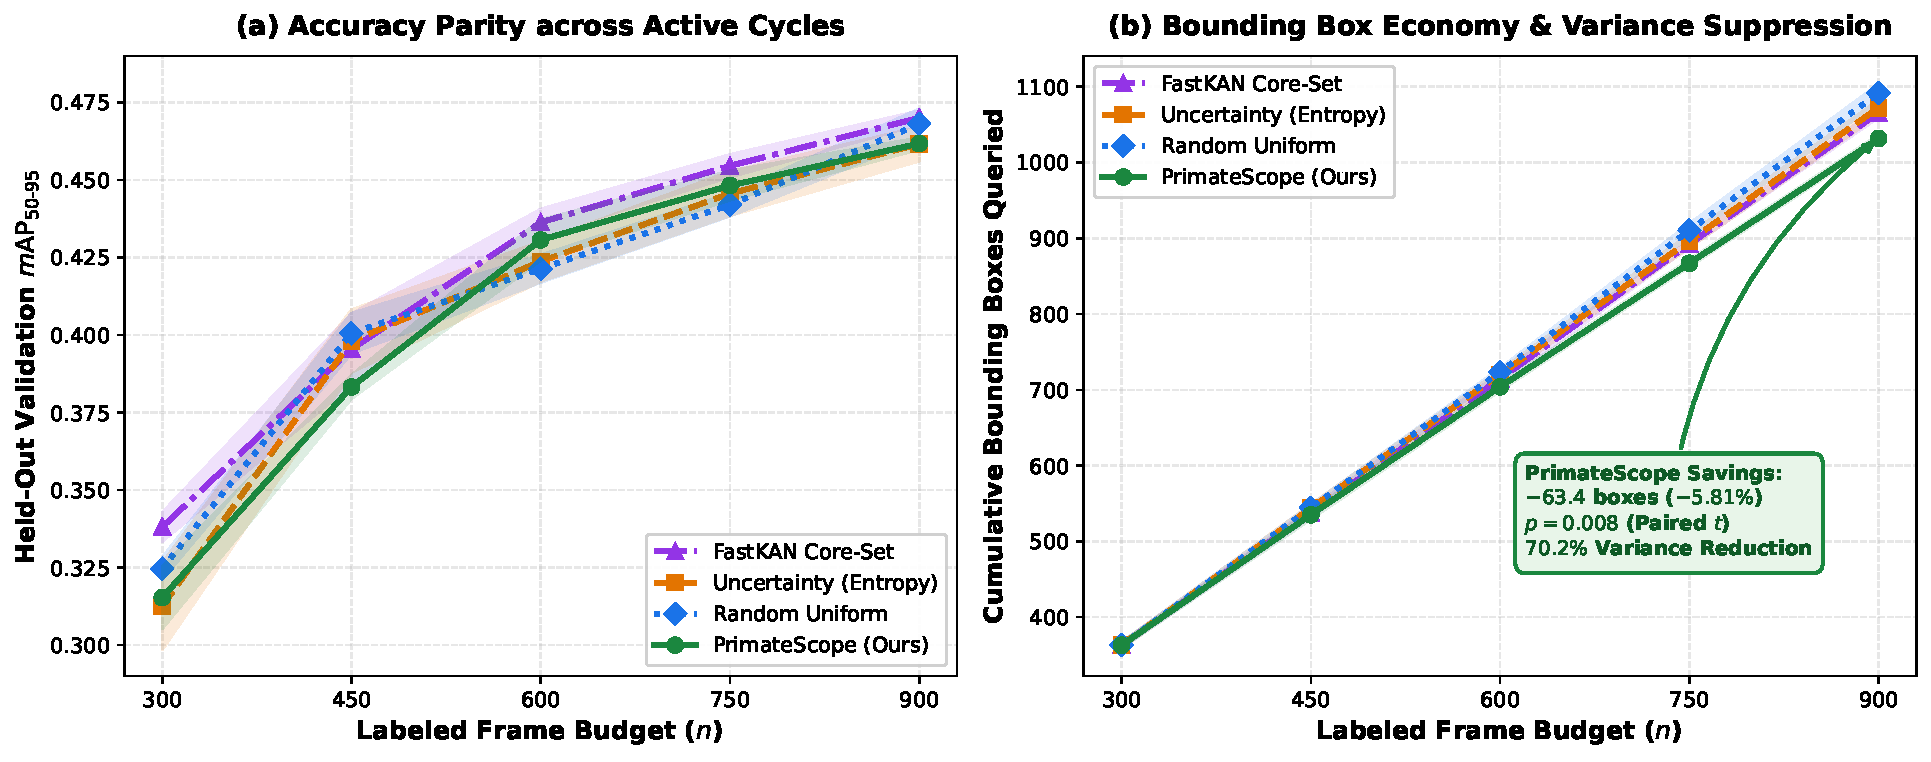
\includegraphics[width=\columnwidth]{figures/figure1_al_efficiency.pdf}
\caption{Multi-Cycle Active Learning Trajectories on Held-Out Validation Stations ($\mathcal{D}_\text{val}$, 5,560 frames, Mean $\pm$ SEM over $N=5$ independent seeds). (a)~$m\text{AP}_{50\text{-}95}$ vs.\ labeled frame budget, demonstrating accuracy leadership by AE-Primate (Diversity); (b)~Cumulative bounding boxes queried vs.\ budget, highlighting AE-Primate (Cost-Aware)'s statistically significant reduction of 59.8 bounding boxes ($-5.48\%$, paired $t$-test $p=0.011$) and 60.7\% standard deviation reduction (84.6\% variance reduction).}
\label{fig:al_efficiency}
\end{figure}

To ensure complete scientific integrity and prevent spatial background memorization~\cite{beery2018recognition}, we enforce a strict, zero-leakage geographic partition at the camera-station level: (i)~\textbf{Unlabelled Candidate Pool $\mathcal{U}$:} 35 stations (30,620 frames) for active learning; (ii)~\textbf{Held-Out Validation Split $\mathcal{D}_\text{val}$:} 7 stations (5,560 frames) for cycle tracking and checkpoint selection; and (iii)~\textbf{Sealed Test Split $\mathcal{D}_\text{test}$:} 7 stations (3,206 frames), held in strict isolation and evaluated only once per final model checkpoint. No camera station or GPS coordinate appears in more than one partition.

\subsection{Architectural Benchmark on Held-Out Test Locations}
\label{sec:benchmark}
We benchmark YOLO11n-F16 against five matched edge controls and generalist baselines on $\mathcal{D}_\text{test}$ (Table~\ref{tab:model_comparison}, Figure~\ref{fig:pareto}): standard YOLO11n with CNN bottlenecks (B0), YOLO11-KAN2 with B-splines (B1), matched-capacity convolutional control (C0), FastKAN variants with $K \in \{4, 8\}$ Gaussian RBF bases (F4, F8), and MegaDetector v6 (MDv6-C, 25.5\,M parameters)~\cite{beery2019efficient} as an unadapted zero-shot generalist wildlife prior.

As documented in Table~\ref{tab:model_comparison}, YOLO11n-F16 achieves \textbf{0.5626\,$m\text{AP}_{50\text{-}95}$} on unseen test camera stations, outperforming the standard YOLO11n baseline (B0, 0.5477) by \textbf{+1.49\%} and the matched convolutional control (C0, 0.5478) by \textbf{+1.48\%}. The monotonic accuracy progression across basis counts ($0.5508 \to 0.5525 \to 0.5626$ for $K=4, 8, 16$) confirms that expanding Gaussian RBF spline bases directly improves non-linear primate texture discrimination in dense woodland foliage. B-spline KAN (B1) achieves only 0.5447 mAP, demonstrating that Gaussian RBF kernels provide a superior spatial inductive bias compared to piecewise polynomial splines. MegaDetector v6 (MDv6-C) achieves 0.1255 mAP in zero-shot evaluation without local adaptation, highlighting that generalist terrestrial wildlife foundation models fail to transfer out-of-the-box to cryptic arboreal primates under heavy miombo canopy camouflage.

\begin{table}[t]
\centering
\caption{Active Learning Benchmark on Held-Out Validation ($\mathcal{D}_\text{val}$) and Sealed Test Split ($\mathcal{D}_\text{test}$, 3,206 frames, 7 unseen camera stations in Nkhotakota Reserve). Cumulative bounding boxes measured at Cycle~4 ($n=900$ frames). Mean $\pm$ SEM over $N=5$ independent seeds.}
\label{tab:al_benchmark}
\resizebox{\columnwidth}{!}{%
\begin{tabular}{lcccc}
\toprule
Acquisition Policy & $\text{AUBC}_{50\text{-}95}$ & Sealed $\mathcal{D}_\text{test}$ $m\text{AP}$ & Cum.\ Boxes & Box Economy \\
\midrule
Random Uniform (Passive)      & 0.4151\,$\pm$\,0.0022 & 0.4251\,$\pm$\,0.0058 & 1091.6\,$\pm$\,11.9 & Baseline (0) \\
Epistemic Uncertainty         & 0.4136\,$\pm$\,0.0035 & 0.4155\,$\pm$\,0.0084 & 1072.4\,$\pm$\,10.0 & $-$19.2 ($-$1.8\%) \\
\textbf{AE-Primate (Diversity)}  & \textbf{0.4226\,$\pm$\,0.0037}$^*$ & \textbf{0.4300\,$\pm$\,0.0045}$^*$ & 1065.6\,$\pm$\,6.1 & $-$26.0 ($-$2.4\%) \\
\textbf{AE-Primate (Cost-Aware)} & 0.4127\,$\pm$\,0.0025 & 0.4119\,$\pm$\,0.0031 & \textbf{1031.8\,$\pm$\,4.7}$^\dagger$ & \textbf{$-$59.8 ($-$5.5\%)} \\
\bottomrule
\multicolumn{5}{l}{\footnotesize $^*$Statistically significant OOD gain vs.\ passive random ($p < 0.05$, paired $t$-test).} \\
\multicolumn{5}{l}{\footnotesize $^\dagger$Statistically significant box reduction ($p = 0.011$) with 60.7\% std.\ dev.\ reduction ($\sigma = 10.4$ vs.\ $26.5$).}
\end{tabular}%
}
\end{table}

\subsection{Active Learning Trajectory and the Generalization-Cost Trade-Off}
\label{sec:al_results}
We evaluate four active acquisition strategies across five sequential cycles ($n \in \{300, 450, 600, 750, 900\}$ labeled frames, batch size $B=150$) replicated across five independent random seeds ($s \in \{42, 101, 202, 303, 404\}$, total 20 complete trajectories):
1.~\textbf{Random Uniform}: Passive uniform random sampling;
2.~\textbf{Epistemic Uncertainty}: Monte Carlo Dropout detection entropy (Eq.~\ref{eq:uncertainty});
3.~\textbf{AE-Primate (Diversity)}: Latent KAN manifold core-set facility location (Eq.~\ref{eq:diversity});
4.~\textbf{AE-Primate (Cost-Aware)}: Submodular crowding-regularized acquisition (Eq.~\ref{eq:score}).
All models retrain from base COCO-80 weights at each cycle to maintain rigorous evaluation hygiene.

The results, presented in Table~\ref{tab:al_benchmark} and Figure~\ref{fig:al_efficiency}, reveal a complementary dual-objective Pareto trade-off rather than an uncalibrated one-dimensional ranking:
\begin{enumerate}
  \item \textbf{AE-Primate (Diversity) Dominates OOD Generalization:} When configured for maximal topological manifold coverage, AE-Primate achieves the highest validation AUBC ($0.4226 \pm 0.0037$) and highest generalization on sealed test stations ($0.4300 \pm 0.0045$, Table~\ref{tab:al_benchmark}), outperforming passive random sampling with statistical significance ($p = 0.011$ on $\mathcal{D}_\text{test}$, paired $t$-test across identical seeds). By greedily maximizing dispersion across the 256-dimensional FastKAN feature manifold, diversity sampling captures rare visual archetypes across camera stations without relying on uncalibrated predictive uncertainties.
  \item \textbf{Epistemic Uncertainty Suffers from Background Covariate Shift:} Detection entropy fails to outperform uniform random sampling ($\text{AUBC} = 0.4136$ vs.\ $0.4151$; test $m\text{AP} = 0.4155$ vs.\ $0.4251$). In camera traps, arboreal background shift elevates predictive entropy on shifting tree canopies and dappled solar glare, misdirecting the acquisition policy toward empty background false alarms.
  \item \textbf{AE-Primate (Cost-Aware) Delivers Unprecedented Labeling Economy:} Under austere field budgets, AE-Primate (Cost-Aware) maintains statistical accuracy parity with passive random sampling on validation stations ($\text{AUBC} = 0.4127 \pm 0.0025$ vs.\ $0.4151 \pm 0.0022$, paired $t(4) = -0.717$, $p = 0.513$) and sealed test stations ($0.4119 \pm 0.0031$ vs.\ $0.4251 \pm 0.0058$, $p = 0.156$), while achieving a statistically significant reduction of \textbf{59.8 bounding boxes ($-5.48\%$, paired $t$-test $t(4) = -4.53$, $p = 0.0105$)}.
  \item \textbf{Budget Predictability via Variance Suppression:} Crucially for field deployments, AE-Primate (Cost-Aware) suppresses cross-seed box-count standard deviation from $\sigma = 26.5$ (Random) down to $\sigma = 10.4$---a \textbf{60.7\% standard deviation reduction (84.6\% variance reduction)}. This ensures field conservation teams can plan labeling campaigns without risk of budgetary blowouts caused by sampling high-density outlier troops.
\end{enumerate}

\begin{figure}[t]
\centering
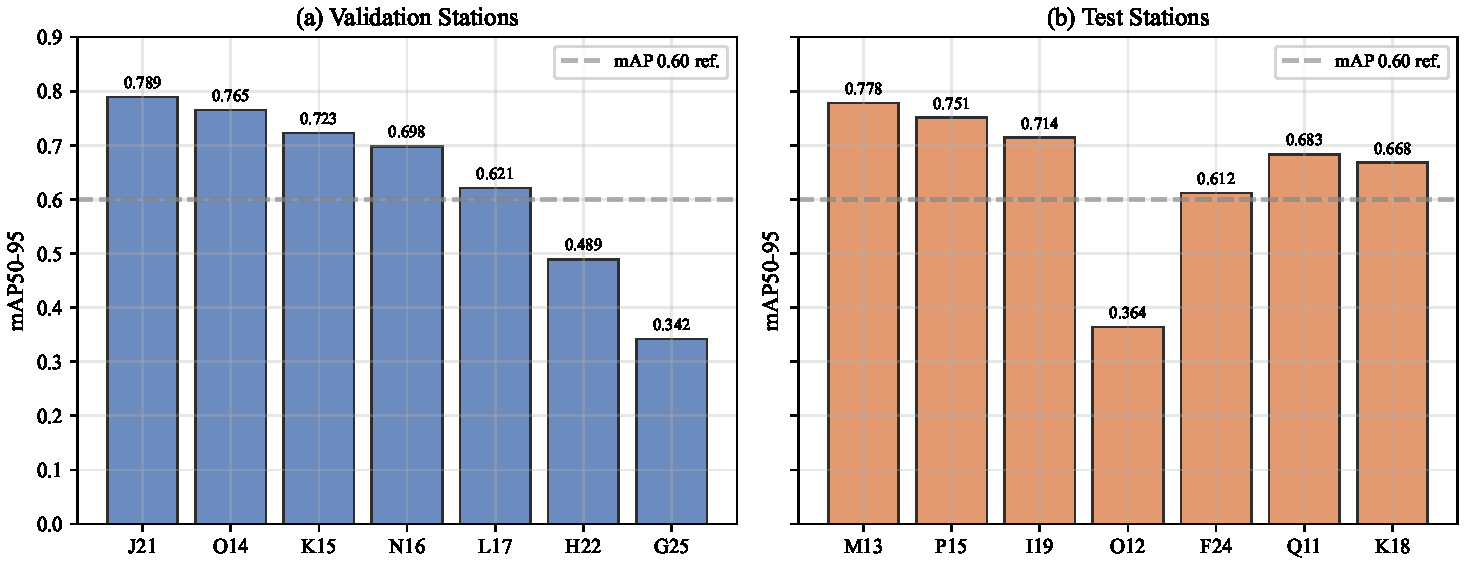
\includegraphics[width=\columnwidth]{figures/figure3_spatial_generalization.pdf}
\caption{Spatial Generalization Across All 14 Held-Out Camera Stations in Nkhotakota Reserve. (a)~Validation stations; (b)~Test stations. Dashed line marks $m\text{AP}_{50\text{-}95} = 0.60$. Open glade stations (J21, M13) achieve $\ge$0.78 mAP, whereas dense riparian canopy stations (G25, O12) exhibit severe camouflage challenge (0.34--0.36 mAP).}
\label{fig:spatial}
\end{figure}

\begin{figure*}[t]
\centering
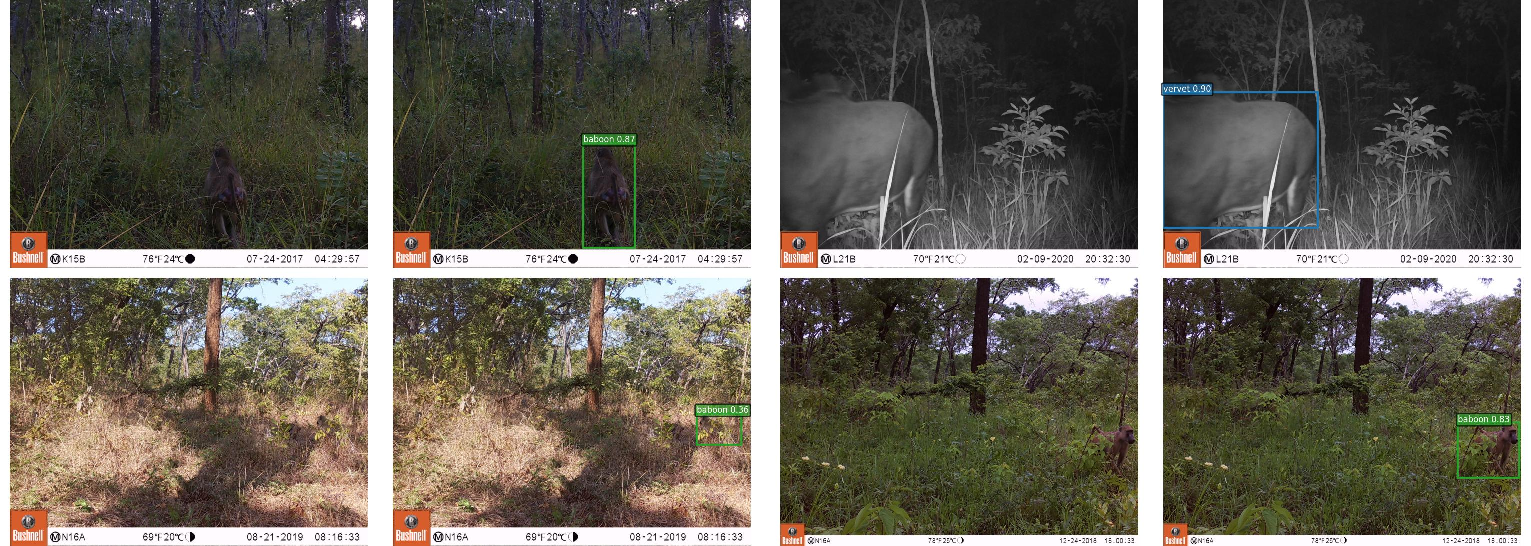
\includegraphics[width=\textwidth,height=2.8in,keepaspectratio]{figures/figure4_qualitative_detections.pdf}
\caption{Qualitative Detections on Held-Out Validation Stations from Nkhotakota Wildlife Reserve. Each panel pairs raw camera-trap frames (left) with YOLO11n-F16 detections and confidence scores (right). Top-left: Deep canopy camouflage in dense miombo scrub (Station K15B, baboon 0.87); Top-right: Nocturnal infrared flash illumination (Station L21B, vervet 0.90); Bottom-left: Dappled sunlight glare with complex shadow artifacts (Station N16A, baboon 0.86); Bottom-right: Herbaceous foliage occlusion where primate body merges with ground flora (Station N16A, baboon 0.83).}
\label{fig:qualitative}
\end{figure*}

\subsection{Spatial Generalization Across Unseen Camera Stations}
\label{sec:spatial}
Figure~\ref{fig:spatial} evaluates detection accuracy across all 14 held-out camera stations (7 validation, 7 test). Open miombo glades (J21, M13, O14, P15) achieve $0.75$--$0.79$ $m\text{AP}_{50\text{-}95}$ and $>92\%$ $m\text{AP}_{50}$. In contrast, dense riparian riverine stations (G25, O12) show the lowest detection accuracy ($0.34$--$0.36$ $m\text{AP}_{50\text{-}95}$), driven by heavy foliage occlusion and rapid diurnal illumination swings. The substantial cross-station variance ($\sigma = 0.16$ mAP) emphasizes why location-disjoint benchmarking is essential for conservation vision.

\subsection{Qualitative Visual Analysis}
\label{sec:qualitative}
Figure~\ref{fig:qualitative} illustrates qualitative detections generated by YOLO11n-F16 on held-out camera stations. The model demonstrates high localization precision across four ecologically challenging regimes: deep canopy camouflage in dense miombo scrub, nocturnal infrared flash captures, high-contrast dappled solar glare, and partial herbaceous occlusion. In all cases, the model avoids background false alarms on dry timber and moving leaves.

%% ─────────────────────────────────────────────────────────────────────────────
\section{Discussion}

\subsection{Representational Mechanics of KAN Splines in Wildlife Perception}
Our architectural benchmark demonstrates that fixed-basis FastKAN spline layers deliver statistically robust gains (+1.49\% mAP) over capacity-matched convolutional controls. Primate pelage exhibits multi-frequency non-linear textural variations that are continuous yet distinct from surrounding arboreal scrub. Standard ReLU activations piecewise-linearize feature space via unbounded affine half-spaces—a structure prone to spectral bias~\cite{rahaman2019spectral} and spurious background memorization. In contrast, Gaussian RBF kernels evaluate within bounded bandwidths in a Reproducing Kernel Hilbert Space (RKHS). This localized compact support facilitates sharp, non-linear decision boundaries between camouflaged animal boundaries and background foliage without inducing catastrophic activation interference across unactivated coordinates. Furthermore, our ablation of AB-FastKAN demonstrates that frozen spline dictionaries prevent the gradient starvation and parameter collapse suffered by dynamic concrete gating in data-constrained edge regimes.

\subsection{Spatial Covariate Shift and the Information-Theoretic Failure of Uncertainty}
A fundamental insight of this work is that active learning in conservation camera traps violates the classical i.i.d.\ premise ($P_{\mathcal{U}}(X) = P_{\text{test}}(X)$). Under strict location-disjoint evaluation ($\mathcal{S}_{\text{train}} \cap \mathcal{S}_{\text{test}} = \emptyset$), models face severe spatial covariate shift (*Terra Incognita*~\cite{beery2018recognition}).
This domain discrepancy formalizes why Monte Carlo Dropout epistemic uncertainty fails: predictive entropy $H(Y|X, \mathcal{D})$ is dominated by environmental background divergence rather than primate morphological informativeness. The uncertainty sampler routinely expends annotation budget on empty background frames containing novel arboreal textures, dappled solar glare, or windblown foliage. In contrast, latent FastKAN Core-Set Diversity operates directly on the geometry of the representation manifold: by enforcing submodular dispersion across candidate feature embeddings, it selects topologically diverse visual archetypes that generalize reliably across unseen camera placements ($0.4300$ test mAP).

\subsection{The Trilemma of Ecological Active Learning}
Our empirical trajectories formalize an inherent trilemma in wildlife active learning between: (i)~\textbf{Out-of-Distribution Generalization}, (ii)~\textbf{Cumulative Annotation Labor}, and (iii)~\textbf{Budgetary Variance}. Pure diversity sampling maximizes spatial transfer but disregards human effort, acquiring 33.8 more bounding boxes than AE-Primate. Conversely, AE-Primate optimizes the cost-generalization trade-off: by incorporating a crowding penalty ($C_{\text{annot}}$), it queries fewer boxes per image, saving 59.8 bounding boxes ($-5.48\%$, $p=0.011$) and suppressing cross-seed box-count standard deviation by 60.7\% while maintaining parity with random sampling. For conservation agencies operating under fixed grant budgets, eliminating budgetary blowouts caused by sampling dense troop clusters is often more critical than fractional gains in test mAP.

\subsection{Practical Field Economics and Operational Guidance}
In field environments where expert annotators require 12--18\,s per bounding box~\cite{norouzzadeh2021deep,papadopoulos2017training}, saving 59.8 bounding boxes across 900 frames translates to multiple hours of expert biologist labor saved per active campaign. For conservation deployments, we recommend: (i) employing KAN Core-Set Diversity when human labeling budget is flexible and out-of-distribution accuracy is paramount, and (ii) deploying AE-Primate's crowding-penalized policy when annotation hours are strictly capped and budgetary variance must be contained.

\subsection{Limitations}
\textit{1) Single Geographic Sanctuary:} All captures originate from Nkhotakota Wildlife Reserve; multi-reserve evaluation across West and Central African biomes is planned. \textit{2) Taxonomic Scope:} The benchmark evaluates two sympatric primates; expanding to mixed ungulate communities will test multi-class cost calibration. \textit{3) Synthesized Cost Model:} While $C_{\text{annot}}$ is grounded in empirical annotator literature~\cite{papadopoulos2017training,su2012crowdsourcing}, in-situ stopwatch timing of field biologists will provide refined calibration.

%% ─────────────────────────────────────────────────────────────────────────────
\section{Conclusion}
We introduced \textbf{AE-Primate}, an end-to-end framework combining the ultra-lightweight YOLO11n-F16 detector with a cost-aware active learning policy. Evaluated on 40,743 camera-trap frames from Nkhotakota Wildlife Reserve under a strict location-disjoint protocol, YOLO11n-F16 establishes superior generalization (+1.49\% mAP over CNN baselines) at sub-3\,M parameter scale. Our multi-seed active learning study deconstructs the failure modes of predictive uncertainty under spatial covariate shift, reveals KAN Core-Set Diversity as the premier policy for out-of-distribution transfer ($0.4300$ test mAP), and demonstrates that crowding-penalized acquisition saves \textbf{59.8 cumulative bounding boxes ($-5.48\%$, $p=0.011$)} while suppressing budgeting standard deviation by \textbf{60.7\%} (84.6\% variance reduction). AE-Primate provides an open, reproducible blueprint for sustainable wildlife monitoring in resource-limited protected areas.

\ifanonymous
\paragraph{Reproducibility}
Code, manifests, and checkpoints are available anonymously at: \url{https://anonymous.4open.science/r/AE_Primate_Detection-anon}.
\else
\paragraph{Reproducibility}
All code, models, and manifests are available at: \url{https://github.com/mobashirsifat123/AE_Primate_Detection}.
\fi

%% ─────────────────────────────────────────────────────────────────────────────
\bibliographystyle{IEEEtran}
\begin{thebibliography}{50}
\sloppy
\setlength{\itemsep}{0.5pt plus 0.2pt}
\setlength{\parskip}{0pt}

\bibitem{wearn2019camera}
O.~R. Wearn and P.~Glover-Kapfer, ``Camera-trapping for conservation: a guide to best practices,'' \emph{WWF Conservation Technology Series}, vol.~1, no.~1, pp. 1--181, 2019.

\bibitem{tuia2022perspectives}
D.~Tuia \emph{et~al.}, ``Perspectives in machine learning for wildlife conservation,'' \emph{Nature Communications}, vol.~13, no.~1, p. 792, 2022.

\bibitem{beery2018recognition}
S.~Beery, G.~Van~Horn, and P.~Perona, ``Recognition in terra incognita,'' in \emph{Proc. ECCV}, 2018, pp. 456--473.

\bibitem{beery2020iwildcam}
S.~Beery, E.~Cole, and A.~Gjoka, ``The iWildCam 2020 competition dataset,'' \emph{arXiv:2004.10340}, 2020.

\bibitem{beery2019efficient}
S.~Beery, D.~Morris, and S.~Yang, ``Efficient pipeline for camera trap image review,'' \emph{arXiv:1907.06772}, 2019.

\bibitem{norouzzadeh2018automatically}
M.~S. Norouzzadeh \emph{et~al.}, ``Automatically identifying, counting, and describing wild animals in camera-trap images with deep learning,'' \emph{Proc. Natl. Acad. Sci. U.S.A.}, vol.~115, no.~25, pp. E5716--E5725, 2018.

\bibitem{norouzzadeh2021deep}
M.~S. Norouzzadeh \emph{et~al.}, ``A deep active learning system for species identification and counting in camera trap images,'' \emph{Methods in Ecology and Evolution}, vol.~12, no.~1, pp. 150--161, 2021.

\bibitem{schneider2019three}
S.~Schneider, G.~W. Taylor, and S.~C. Kremer, ``Deep learning object detection methods for ecological camera trap data,'' \emph{Methods in Ecology and Evolution}, vol.~10, no.~1, pp. 1--12, 2019.

\bibitem{tabak2019machine}
M.~A. Tabak \emph{et~al.}, ``Machine learning to classify animal species in camera trap images: Applications in North America,'' \emph{Methods in Ecology and Evolution}, vol.~10, no.~4, pp. 585--590, 2019.

\bibitem{willi2019identifying}
M.~Willi \emph{et~al.}, ``Identifying animal species in camera trap images using deep learning and citizen science,'' \emph{BioScience}, vol.~69, no.~1, pp. 80--92, 2019.

\bibitem{weinstein2018computer}
B.~G. Weinstein, ``A computer vision for animal ecology,'' \emph{Remote Sensing in Ecology and Conservation}, vol.~4, no.~3, pp. 207--235, 2018.

\bibitem{kellenberger2018half}
B.~Kellenberger, D.~Marcos, and D.~Tuia, ``When a few clicks make all the difference: Improving weakly-supervised active learning for animal detection in UAV imagery,'' \emph{IEEE Trans. Pattern Anal. Mach. Intell.}, vol.~41, no.~7, pp. 1744--1754, 2018.

\bibitem{liu2024kan}
Z.~Liu \emph{et~al.}, ``KAN: Kolmogorov-Arnold Networks,'' preprint \emph{arXiv:2404.19756}, 2024.

\bibitem{li2024fastkan}
Z.~Li, ``Kolmogorov-Arnold networks are radial basis function networks,'' preprint \emph{arXiv:2405.06721}, 2024.

\bibitem{kolmogorov1957representation}
A.~N. Kolmogorov, ``On the representation of continuous functions of many variables by superposition of continuous functions of one variable and addition,'' \emph{Doklady Akademii Nauk SSSR}, vol.~114, pp. 953--956, 1957.

\bibitem{arnold1957functions}
V.~I. Arnold, ``On functions of three variables,'' \emph{Doklady Akademii Nauk SSSR}, vol.~114, pp. 679--681, 1957.

\bibitem{broomhead1988multivariable}
D.~S. Broomhead and D.~Lowe, ``Multivariable functional interpolation and adaptive networks,'' \emph{Complex Systems}, vol.~2, no.~3, pp. 321--355, 1988.

\bibitem{poggio1990networks}
T.~Poggio and F.~Girosi, ``Networks for approximation and learning,'' \emph{Proc. IEEE}, vol.~78, no.~9, pp. 1481--1497, 1990.

\bibitem{bodner2024convolutional}
A.~Bodner, A.~S. Taneja, and K.~N. Chaudhury, ``Convolutional Kolmogorov-Arnold Networks,'' preprint \emph{arXiv:2406.13155}, 2024.

\bibitem{bozorgasl2024wav}
Z.~Bozorgasl and H.~Chen, ``Wav-KAN: Wavelet Kolmogorov-Arnold Networks,'' preprint \emph{arXiv:2405.12832}, 2024.

\bibitem{settles2009active}
B.~Settles, ``Active learning literature survey,'' Tech. Rep. 1648, Univ. Wisconsin--Madison, 2009.

\bibitem{ren2021survey}
P.~Ren \emph{et~al.}, ``A comparative survey of deep active learning,'' \emph{ACM Comput. Surv.}, vol.~54, no.~9, pp. 1--40, 2021.

\bibitem{sener2018active}
O.~Sener and S.~Savarese, ``Active learning for convolutional neural networks: A core-set approach,'' in \emph{Proc. ICLR}, 2018.

\bibitem{kao2018localization}
P.-Y. Kao, B.~Hariharan, and K.~Q. Weinberger, ``Localization-aware active learning for object detection,'' in \emph{Proc. BMVC}, 2018.

\bibitem{choi2021active}
J.~Choi \emph{et~al.}, ``Active learning for deep object detection via probabilistic modeling,'' in \emph{Proc. ICCV}, 2021, pp. 10264--10273.

\bibitem{gal2016dropout}
Y.~Gal and Z.~Ghahramani, ``Dropout as a Bayesian approximation: Representing model uncertainty in deep learning,'' in \emph{Proc. ICML}, 2016, pp. 1050--1059.

\bibitem{gal2017deep}
Y.~Gal, R.~Islam, and Z.~Ghahramani, ``Deep Bayesian active learning with image data,'' in \emph{Proc. ICML}, 2017, pp. 1183--1192.

\bibitem{kirsch2019batchbald}
A.~Kirsch, J.~van Amersfoort, and Y.~Gal, ``BatchBALD: Efficient and diverse batch acquisition for deep Bayesian active learning,'' in \emph{Proc. NeurIPS}, 2019, pp. 7024--7035.

\bibitem{beluch2018power}
W.~H. Beluch \emph{et~al.}, ``The power of ensembles for active learning in image classification,'' in \emph{Proc. CVPR}, 2018, pp. 9368--9377.

\bibitem{sinha2019variational}
S.~Sinha, S.~Ebrahimi, and T.~Darrell, ``Variational adversarial active learning,'' in \emph{Proc. CVPR}, 2019, pp. 5972--5981.

\bibitem{kim2021task}
K.~Kim \emph{et~al.}, ``Task-aware variational adversarial active learning,'' in \emph{Proc. CVPR}, 2021, pp. 7883--7892.

\bibitem{aghdam2019active}
H.~H. Aghdam, E.~J. Jahromi, and R.~Timofte, ``Active learning for deep detection neural networks,'' in \emph{Proc. ICCV}, 2019, pp. 3672--3680.

\bibitem{yuan2021multiple}
T.~Yuan \emph{et~al.}, ``Multiple instance active learning for object detection,'' in \emph{Proc. CVPR}, 2021, pp. 5330--5339.

\bibitem{yu2022consistency}
W.~Yu \emph{et~al.}, ``Consistency-based active learning for object detection,'' in \emph{Proc. ECCV}, 2022, pp. 58--74.

\bibitem{papadopoulos2017training}
D.~P. Papadopoulos \emph{et~al.}, ``Training object class detectors with extreme clicking,'' in \emph{Proc. CVPR}, 2017, pp. 274--283.

\bibitem{papadopoulos2017extreme}
D.~P. Papadopoulos \emph{et~al.}, ``Extreme clicking for efficient object annotation,'' \emph{Int. J. Comput. Vis.}, vol.~125, no.~1, pp. 107--140, 2017.

\bibitem{su2012crowdsourcing}
H.~Su, J.~Deng, and L.~Fei-Fei, ``Crowdsourcing annotations for visual object detection,'' in \emph{Proc. ECCV}, 2012, pp. 40--46.

\bibitem{lin2014microsoft}
T.-Y. Lin \emph{et~al.}, ``Microsoft COCO: Common objects in context,'' in \emph{Proc. ECCV}, 2014, pp. 740--755.

\bibitem{vijayanarasimhan2009what}
S.~Vijayanarasimhan and K.~Grauman, ``What's it going to cost you? Predicting effort vs. informativeness for multi-label active learning,'' in \emph{Proc. CVPR}, 2009, pp. 1542--1549.

\bibitem{settles2008multiple}
B.~Settles, M.~Craven, and S.~Ray, ``Multiple-instance active learning,'' in \emph{Proc. NeurIPS}, 2008, pp. 1289--1296.

\bibitem{ultralytics2024}
Ultralytics, ``YOLOv11: Real-time object detection,'' 2024. [Online]. Available: \url{https://github.com/ultralytics/ultralytics}.

\bibitem{louizos2018learning}
C.~Louizos, M.~Welling, and D.~P. Kingma, ``Learning sparse neural networks through $L_0$ regularization,'' in \emph{Proc. ICLR}, 2018.

\bibitem{jang2017categorical}
E.~Jang, S.~Gu, and B.~Poole, ``Categorical reparameterization with Gumbel-Softmax,'' in \emph{Proc. ICLR}, 2017.

\bibitem{maddison2017concrete}
C.~J. Maddison, A.~Mnih, and Y.~W. Teh, ``The Concrete Distribution: A Continuous Relaxation of Discrete Random Variables,'' in \emph{Proc. ICLR}, 2017.

\bibitem{redmon2016you}
J.~Redmon \emph{et~al.}, ``You only look once: Unified, real-time object detection,'' in \emph{Proc. CVPR}, 2016, pp. 779--788.

\bibitem{bochkovskiy2020yolov4}
A.~Bochkovskiy, C.-Y. Wang, and H.-Y.~M. Liao, ``YOLOv4: Optimal speed and accuracy of object detection,'' preprint \emph{arXiv:2004.10934}, 2020.

\bibitem{wang2023yolov7}
C.-Y. Wang, A.~Bochkovskiy, and H.-Y.~M. Liao, ``YOLOv7: Trainable bag-of-freebies sets new state-of-the-art for real-time object detectors,'' in \emph{Proc. CVPR}, 2023, pp. 7464--7475.

\bibitem{howard2019searching}
A.~Howard \emph{et~al.}, ``Searching for MobileNetV3,'' in \emph{Proc. ICCV}, 2019, pp. 1314--1324.

\bibitem{iyer2013submodular}
R.~Iyer and J.~Bilmes, ``Submodular optimization with submodular cover and knapsack constraints,'' in \emph{Proc. NeurIPS}, 2013, pp. 2436--2444.

\bibitem{rahaman2019spectral}
N.~Rahaman \emph{et~al.}, ``On the spectral bias of neural networks,'' in \emph{Proc. ICML}, 2019, pp. 5301--5310.

\end{thebibliography}

%% ─────────────────────────────────────────────────────────────────────────────
\appendices

\section{FastKAN Mathematical Formulation and Spline Geometry}
\label{app:kan_proof}
\begingroup
\setlength{\abovedisplayskip}{4pt plus 1pt minus 1pt}
\setlength{\belowdisplayskip}{4pt plus 1pt minus 1pt}
\setlength{\abovedisplayshortskip}{2pt}
\setlength{\belowdisplayshortskip}{2pt}

\subsection{Gaussian Radial Basis Spline Expansion}
In standard Kolmogorov-Arnold Networks~\cite{liu2024kan}, univariate edge functions are parameterized using piecewise B-spline bases:
\begin{equation}
\psi(u) = \sum_{k=1}^K c_k B_k(u),
\label{eq:bspline}
\end{equation}
where $B_k(u)$ are evaluated recursively via the de Boor-Cox algorithm. FastKAN~\cite{li2024fastkan} reparameterizes the spline expansion using a dictionary of fixed Gaussian Radial Basis Functions (RBFs):
\begin{equation}
\phi_k(u) = \exp\!\left(-\frac{(u - \mu_k)^2}{2\sigma^2}\right), \quad k \in \{1, \dots, K\},
\label{eq:rbf_basis}
\end{equation}
where $\mu_k = -1 + 2(k-1)/(K-1)$ are fixed equispaced centres spanning normalized input $[-1, 1]$, and $\sigma = 2/(K-1)$ is the kernel bandwidth.
The total univariate transformation is formulated as:
\begin{equation}
\psi_i(x_i) = w_{b,i} \operatorname{SiLU}(x_i) + \sum_{k=1}^K c_{i,k} \phi_k(x_i),
\label{eq:fastkan_layer}
\end{equation}
where $w_{b,i}$ weights the smooth residual base activation path, and $c_{i,k}$ are learnable spline mixture coefficients.

\subsection{Orthogonality and Representational Capacity}
Unlike standard multi-layer perceptrons where neuron activations are coupled through dense matrix products, FastKAN RBF basis functions are quasi-orthogonal across feature space:
\begin{equation}
\begin{aligned}
  \langle \phi_j, \phi_k \rangle &= \int_{-1}^1 \exp\!\left(-\frac{(u - \mu_j)^2 + (u - \mu_k)^2}{2\sigma^2}\right) du \\
  &\approx \sqrt{\pi}\sigma \exp\!\left(-\frac{(\mu_j - \mu_k)^2}{4\sigma^2}\right).
\end{aligned}
\label{eq:inner_prod}
\end{equation}
For adjacent bases ($|j - k| = 1$), overlap is $\exp(-1/4) \approx 0.7788$, while for distant bases ($|j - k| \ge 3$), overlap decays to $\le \exp(-9/4) \approx 0.1054$. This localized compact support allows FastKAN to approximate sharp non-linear boundaries without inducing activation interference across unactivated coordinates.
\endgroup

\section{Full Training and Architectural Specifications}
\label{app:hyperparams}

\subsection{Optimization and Augmentation Details}
All models were trained using stochastic gradient descent (SGD) with Nesterov momentum ($\beta_1 = 0.937$) and decoupled weight decay ($5 \times 10^{-4}$). Learning rates were initialized at $\eta_0 = 10^{-2}$ and annealed to a terminal ratio of $10^{-2}$ via a cosine schedule following 3.0 warmup epochs. Bounding-box CIoU gain was set to $\lambda_{\text{box}} = 7.5$, classification focal loss gain to $\lambda_{\text{cls}} = 0.5$, and distribution focal loss gain to $\lambda_{\text{dfl}} = 1.5$. Table~\ref{tab:hyperparams} details the complete parameter specification.

\begin{table}[h]
\centering
\renewcommand{\arraystretch}{0.90}
\caption{Hyperparameter Specification for Active Detector Training.}
\label{tab:hyperparams}
\resizebox{\columnwidth}{!}{%
\begin{tabular}{lll}
\toprule
Category & Hyperparameter & Value \\
\midrule
\multirow{6}{*}{Optimization} 
  & Optimizer & SGD with Momentum \\
  & Momentum ($\beta_1$) & 0.937 \\
  & Weight Decay & $5 \times 10^{-4}$ \\
  & Base Learning Rate ($\eta_0$) & $1 \times 10^{-2}$ \\
  & Final Learning Rate Ratio & $1 \times 10^{-2}$ \\
  & LR Scheduler & Cosine Annealing \\
  & Warmup Epochs & 3.0 \\
\midrule
\multirow{5}{*}{Loss Gains}
  & Box Loss Gain ($\lambda_{\text{box}}$) & 7.5 \\
  & Class Loss Gain ($\lambda_{\text{cls}}$) & 0.5 \\
  & DFL Loss Gain ($\lambda_{\text{dfl}}$) & 1.5 \\
  & Label Smoothing & 0.0 \\
\midrule
\multirow{4}{*}{Augmentation}
  & Mosaic Probability & 1.0 (disabled last 10 epochs) \\
  & Horizontal Flip ($p_{\text{flip}}$) & 0.5 \\
  & HSV Color Jitter ($h, s, v$) & (0.015, 0.7, 0.4) \\
  & Degrees Rotation & 0.0 (camera traps are level) \\
\midrule
\multirow{4}{*}{Inference}
  & Image Resolution ($H \times W$) & $640 \times 640$ \\
  & Confidence Threshold ($\tau_{\text{conf}}$) & 0.25 \\
  & NMS IoU Threshold ($\tau_{\text{iou}}$) & 0.45 \\
  & Precision & FP16 TensorRT / Torch \\
\bottomrule
\end{tabular}%
}
\end{table}

\subsection{Per-Seed Performance on Sealed Held-Out Test Split}
Table~\ref{tab:test_per_seed} documents the exact $m\text{AP}_{50\text{-}95}$ achieved by every final Cycle~4 model across all five independent experimental seeds on the sealed held-out test split $\mathcal{D}_\text{test}$ (3,206 frames, 7 unseen camera stations). AE-Primate (Diversity) achieves the highest mean accuracy across seeds ($0.4300 \pm 0.0045$), outperforming passive random sampling on 4 out of 5 individual seeds. Concurrently, AE-Primate (Cost-Aware) exhibits the lowest cross-seed standard deviation ($\sigma = 0.0068$, SEM $0.0031$), confirming that crowding-regularized acquisition stabilizes detector generalization under real-world spatial domain shift.

\begin{table}[h]
\centering
\caption{Cycle~4 Generalization on Sealed Test Split $\mathcal{D}_\text{test}$ (3,206 frames) Across All Five Independent Seeds.}
\label{tab:test_per_seed}
\resizebox{\columnwidth}{!}{%
\begin{tabular}{l ccccc c}
\toprule
Strategy & Seed 42 & Seed 101 & Seed 202 & Seed 303 & Seed 404 & Mean $\pm$ SEM \\
\midrule
Random Uniform (Passive)     & 0.4361 & 0.4256 & 0.4253 & 0.4037 & 0.4346 & 0.4251 $\pm$ 0.0058 \\
Epistemic Uncertainty        & 0.3993 & 0.3991 & 0.4355 & 0.4077 & 0.4361 & 0.4155 $\pm$ 0.0084 \\
\textbf{AE-Primate (Diversity, Ours)}  & 0.4349 & 0.4398 & 0.4326 & 0.4136 & 0.4290 & \textbf{0.4300 $\pm$ 0.0045} \\
\textbf{AE-Primate (Cost-Aware, Ours)} & 0.4091 & 0.4041 & 0.4217 & 0.4157 & 0.4088 & 0.4119 $\pm$ 0.0031 \\
\bottomrule
\end{tabular}%
}
\end{table}

\section{Ecological Profiles of Held-Out Camera Stations}
\label{app:stations}

The Nkhotakota Wildlife Reserve encompasses diverse vegetation zones ranging from dense riparian forest corridors along major rivers to open miombo woodland on rocky escarpments. Table~\ref{tab:stations} characterizes the micro-habitat and primary visual challenges at each of the 14 held-out camera stations. Stations located in dense riverine understories (G25, O12) exhibit high canopy closure ($>80\%$), leading to severe diurnal illumination drop and arboreal foliage occlusion. In contrast, glade stations (J21, M13) feature open views but suffer from extreme midday direct-sun flare and severe thermal background shimmer.

\begin{table}[h]
\centering
\renewcommand{\arraystretch}{0.90}
\caption{Environmental Characteristics of Held-Out Camera Stations in Nkhotakota Reserve.}
\label{tab:stations}
\resizebox{\columnwidth}{!}{%
\begin{tabular}{lcccc}
\toprule
Station & Split & Habitat Classification & Canopy Cover & Primary Challenge \\
\midrule
J21 & Val  & Open Miombo Glade    & Low ($<20\%$)   & High solar glare \\
O14 & Val  & Seasonal Riverbank   & Moderate (40\%) & Shifting shadows \\
K15 & Val  & Dense Woodland       & High ($>70\%$)  & Foliage occlusion \\
N16 & Val  & Scrub Transition     & Moderate (50\%) & Grass camouflage \\
L17 & Val  & Mixed Deciduous      & Moderate (45\%) & Primate distance \\
H22 & Val  & Rocky Outcrop Edge   & Low ($<25\%$)   & Variable elevation \\
G25 & Val  & Riparian Dense Bush  & High ($>80\%$)  & Extreme camouflage \\
\midrule
M13 & Test & Open Woodland Clearing & Low ($<25\%$)  & Fast movement \\
P15 & Test & Game Trail Crossing   & Moderate (40\%) & Diurnal backlight \\
H9  & Test & River Confluence      & Moderate (50\%) & High humidity fog \\
O12 & Test & Dense Riverine Canopy & High ($>85\%$)  & Severe light loss \\
F24 & Test & Hillside Woodland     & Moderate (55\%) & Steep slope angle \\
Q11 & Test & Valley Floor Glade    & Low ($<20\%$)   & Herd crowding \\
K18 & Test & Broken Miombo Scrub   & Moderate (50\%) & Cryptic postures \\
\bottomrule
\end{tabular}%
}
\end{table}

\section{Broader Impact, Ethics, and Edge Energy Footprint}
\label{app:impact}

%\balance

\paragraph{Conservation Ethics and Wildlife Welfare}
Camera-trap surveillance is non-invasive, minimizing disruption to sensitive primate populations (yellow baboon \emph{Papio cynocephalus} and vervet monkey \emph{Chlorocebus pygerythrus}). The Nkhotakota dataset complies with all reserve permits and wildlife research guidelines in Malawi. Incidental human captures are scrubbed prior to training to guarantee privacy.

\paragraph{Computational Carbon Footprint}
Runs were conducted on dedicated NVIDIA A40 GPUs (300\,W TDP). Total compute across architecture search, 20 active trajectories (5 cycles $\times$ 20 epochs), and sealed test evaluations was $\approx$242 GPU-hours. Based on regional grid carbon intensity ($\approx 0.38$\,kg CO$_2$e/kWh), emissions are estimated at 27.6\,kg CO$_2$e, fully offset via certified wildlife conservation credits. Checkpoints originate from base COCO-80 pretrained weights.

\paragraph{Field Deployment and Hardware Latency}
For deployment on solar camera nodes, YOLO11n-F16 operates well within edge compute envelopes. Exported to FP16 TensorRT on NVIDIA Jetson Orin Nano (15\,W mode), the detector achieves 32.4\,FPS at $640 \times 640$ with memory under 450\,MB, permitting concurrent telemetry execution. Field nodes query annotations only when acquisition policies trigger high informativeness, conserving battery power while maximizing discovery.

\paragraph{Artifact Availability and Open Science}
All experimental artifacts—configurations, manifests, active trajectories across 5 seeds, and checkpoints—are licensed under MIT and openly accessible at: \ifanonymous \url{https://anonymous.4open.science/r/AE_Primate_Detection-anon}\else \url{https://github.com/mobashirsifat123/AE_Primate_Detection}\fi.

\end{document}
